

\tikzset{every picture/.style={line width=0.75pt}} %set default line width to 0.75pt        

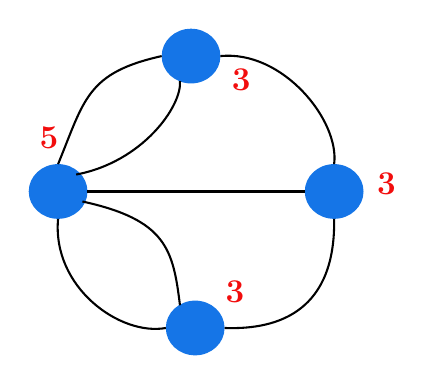
\begin{tikzpicture}[x=0.75pt,y=0.75pt,yscale=-1,xscale=1]
%uncomment if require: \path (0,177); %set diagram left start at 0, and has height of 177

%Shape: Ellipse [id:dp8878451264053866] 
\draw  [draw opacity=0][fill={rgb, 255:red, 21; green, 117; blue, 231 }  ,fill opacity=1 ] (68.33,18.19) .. controls (68.33,10.9) and (74.66,5) .. (82.48,5) .. controls (90.29,5) and (96.63,10.9) .. (96.63,18.19) .. controls (96.63,25.47) and (90.29,31.37) .. (82.48,31.37) .. controls (74.66,31.37) and (68.33,25.47) .. (68.33,18.19) -- cycle ;
%Shape: Ellipse [id:dp2916294149093952] 
\draw  [draw opacity=0][fill={rgb, 255:red, 21; green, 117; blue, 231 }  ,fill opacity=1 ] (137.27,83.42) .. controls (137.27,76.13) and (143.61,70.23) .. (151.42,70.23) .. controls (159.24,70.23) and (165.58,76.13) .. (165.58,83.42) .. controls (165.58,90.7) and (159.24,96.6) .. (151.42,96.6) .. controls (143.61,96.6) and (137.27,90.7) .. (137.27,83.42) -- cycle ;
%Shape: Ellipse [id:dp3230435826467881] 
\draw  [draw opacity=0][fill={rgb, 255:red, 21; green, 117; blue, 231 }  ,fill opacity=1 ] (70.33,149.19) .. controls (70.33,141.9) and (76.66,136) .. (84.48,136) .. controls (92.29,136) and (98.63,141.9) .. (98.63,149.19) .. controls (98.63,156.47) and (92.29,162.37) .. (84.48,162.37) .. controls (76.66,162.37) and (70.33,156.47) .. (70.33,149.19) -- cycle ;
%Shape: Ellipse [id:dp43124705110127093] 
\draw  [draw opacity=0][fill={rgb, 255:red, 21; green, 117; blue, 231 }  ,fill opacity=1 ] (4.27,83.42) .. controls (4.27,76.13) and (10.61,70.23) .. (18.42,70.23) .. controls (26.24,70.23) and (32.58,76.13) .. (32.58,83.42) .. controls (32.58,90.7) and (26.24,96.6) .. (18.42,96.6) .. controls (10.61,96.6) and (4.27,90.7) .. (4.27,83.42) -- cycle ;
%Curve Lines [id:da2175749921862662] 
\draw    (18.42,70.23) .. controls (31.15,39.25) and (32.15,26.25) .. (68.33,18.19) ;
%Curve Lines [id:da3475393637016071] 
\draw    (70.33,149.19) .. controls (48.33,153.19) and (15.42,129.6) .. (18.42,96.6) ;
%Curve Lines [id:da8464775768749004] 
\draw    (77.15,138.25) .. controls (73.83,111.49) and (70.73,97.08) .. (30.15,88.25) ;
%Curve Lines [id:da2560797041651943] 
\draw    (27.15,75.25) .. controls (59.15,69.25) and (78.15,42.25) .. (77.15,30.25) ;
%Curve Lines [id:da7980507121214329] 
\draw    (151.42,70.23) .. controls (154.15,49.25) and (126.63,15.19) .. (96.63,18.19) ;
%Curve Lines [id:da8344460663280768] 
\draw    (151.42,96.6) .. controls (152.15,140.25) and (125.63,150.19) .. (98.63,149.19) ;
%Straight Lines [id:da00593623081886796] 
\draw    (32.58,83.42) -- (137.27,83.42) ;

% Text Node
\draw (8,51) node [anchor=north west][inner sep=0.75pt]  [font=\large] [align=left] {\textbf{\textcolor[rgb]{0.95,0.05,0.05}{5}}};
% Text Node
\draw (100.63,23.19) node [anchor=north west][inner sep=0.75pt]  [font=\large] [align=left] {\textbf{\textcolor[rgb]{0.95,0.05,0.05}{3}}};
% Text Node
\draw (170.63,73.19) node [anchor=north west][inner sep=0.75pt]  [font=\large] [align=left] {\textbf{\textcolor[rgb]{0.95,0.05,0.05}{3}}};
% Text Node
\draw (97.63,125.19) node [anchor=north west][inner sep=0.75pt]  [font=\large] [align=left] {\textbf{\textcolor[rgb]{0.95,0.05,0.05}{3}}};


\end{tikzpicture}